\documentclass[table]{beamer}
\usepackage[utf8]{inputenc}
\usepackage[brazilian]{babel}
\usepackage{amsmath}
\usepackage{graphicx}
\usepackage{hyperref}
\usepackage{ragged2e}   
\usepackage{epstopdf}
\usepackage{multirow}
\usepackage{minted}
\usepackage{booktabs}

\setbeamertemplate{sidebar right}{}
\setbeamertemplate{footline}{%
\hfill\usebeamertemplate***{navigation symbols}
\hspace{1cm}\insertframenumber{}/\inserttotalframenumber}

\addtobeamertemplate{block begin}{}{\justifying}  %new code

\setbeamertemplate{footline}
{
  \leavevmode%
  \hbox{%
  \begin{beamercolorbox}[wd=.333333\paperwidth,ht=2.25ex,dp=1ex,center]{author in head/foot}%
    \usebeamerfont{author in head/foot}\insertsection
  \end{beamercolorbox}%
  \begin{beamercolorbox}[wd=.333333\paperwidth,ht=2.25ex,dp=1ex,center]{title in head/foot}%
    \usebeamerfont{title in head/foot}\insertsubsection
  \end{beamercolorbox}%
  \begin{beamercolorbox}[wd=.333333\paperwidth,ht=2.25ex,dp=1ex,right]{date in head/foot}%
    \usebeamerfont{date in head/foot}\insertshortdate{}\hspace*{2em}
    \insertframenumber{} / \inserttotalframenumber\hspace*{2ex} 
  \end{beamercolorbox}}%
  \vskip0pt%
}

\begin{document}

\begin{frame}
   \frametitle{Compiladores}
   \large
   \begin{center}
      Visão Geral do Processo de Compilação 
   \end{center}
   \scriptsize
   \begin{center}
      João Marcelo Uchôa de Alencar \\
      joao.marcelo@ufc.br \\
      UFC-Quixadá
   \end{center}
\end{frame}

\begin{frame}
   \tableofcontents
\end{frame}

\begin{frame}
   \frametitle{Visão Geral}
   \centering
   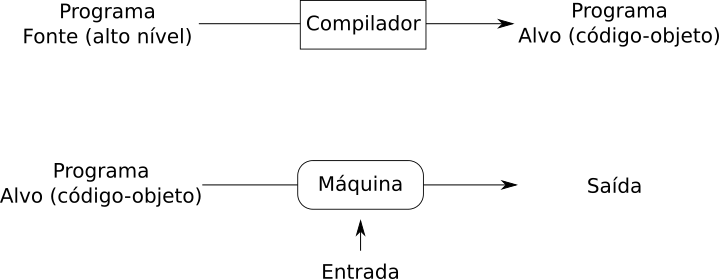
\includegraphics[width=\linewidth,height=\textheight,keepaspectratio]{figuras/visaogeralcompilacao.png}<1>
   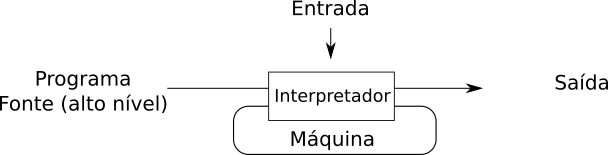
\includegraphics[width=\linewidth,height=\textheight,keepaspectratio]{figuras/visaogeralinterpretacao.png}<2>
   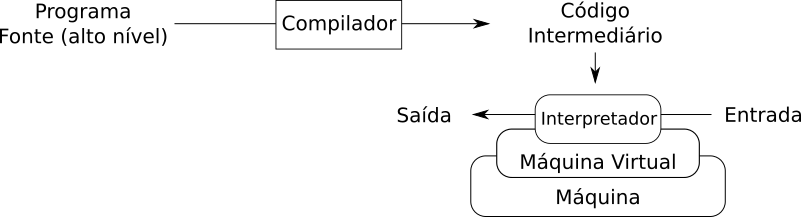
\includegraphics[width=\linewidth,height=\textheight,keepaspectratio]{figuras/visaogeralvm.png}<3>
\end{frame}


\begin{frame}
   \frametitle{Reflexões}
   \begin{itemize}
      \item Qual é a diferença entre um compilador e interpretador?
      \item Quais as vantagens/desvantagens de cada um?
      \item Um compilador que ao receber uma linguagem de alto nível produza código em C no lugar de código objeto teria alguma utilidade?
   \end{itemize}
\end{frame}

\section{Histórico}

\begin{frame}
   \frametitle{Histórico}
   \begin{columns}
      \begin{column}{0.5\textwidth}
         \begin{block}{Linguagem de Máquina}
         C7 06 0000 0002
         \end{block}

         \begin{block}{Linguagem de Montagem}
         MOV X, 2
         \end{block}

         \begin{block}{Linguagem de Alto Nível}
         x = 2;
         \end{block}
      \end{column}
      \begin{column}{0.5\textwidth}
         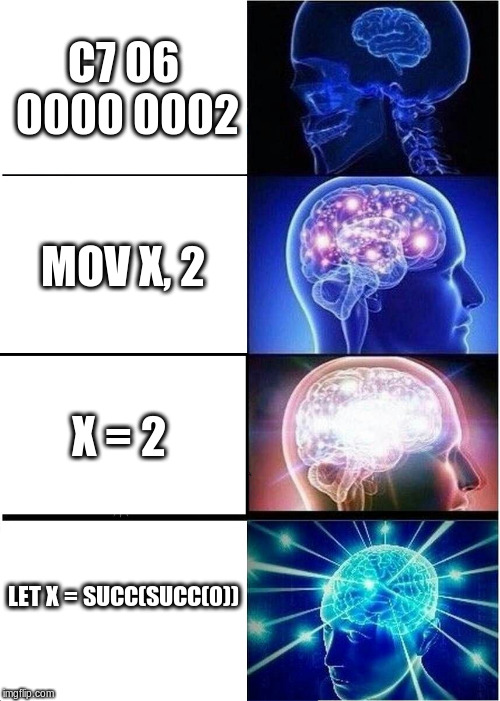
\includegraphics[scale=0.3]{figuras/expandingbrain.jpg}
      \end{column}
   \end{columns}

\end{frame}

\begin{frame}
   \frametitle{Histórico}
   \begin{itemize}
      \item John Backus: Fortran;
      \item Noam Chomsky: Gramáticas;
      \item Geradores de analisadores sintáticos e geradores de sistemas de varredura;
      \item Verificação de tipos e linguagens funcionais.
   \end{itemize}
\end{frame}

\begin{frame}[fragile]
   \frametitle{Exemplo - Linguagem de Alto Nível}
   \begin{minted}{c}
#include <stdio.h>

int main(int argc, char *argv[]) {
   int x = 2;
   return 0;
}
   \end{minted}
\end{frame}

\begin{frame}[fragile]
   \frametitle{Exemplo - Linguagem de Montagem}
   \scriptsize
   \begin{minted}{c}
	.file	"historico.c"
	.text
	.globl	main
	.type	main, @function
main:
.LFB0:
	.cfi_startproc
	pushq	%rbp
	.cfi_def_cfa_offset 16
	.cfi_offset 6, -16
	movq	%rsp, %rbp
	.cfi_def_cfa_register 6
	movl	%edi, -20(%rbp)
	movq	%rsi, -32(%rbp)
	movl	$2, -4(%rbp)
	movl	$0, %eax
	popq	%rbp
	.cfi_def_cfa 7, 8
	ret
	.cfi_endproc
.LFE0:
	.size	main, .-main
	.ident	"GCC: (Ubuntu 5.4.0-6ubuntu1~16.04.6) 5.4.0 20160609"
	.section	.note.GNU-stack,"",@progbits
   \end{minted}
\end{frame}

\section{Programas Relacionados}

\begin{frame}
   \frametitle{Programas Relacionados}
   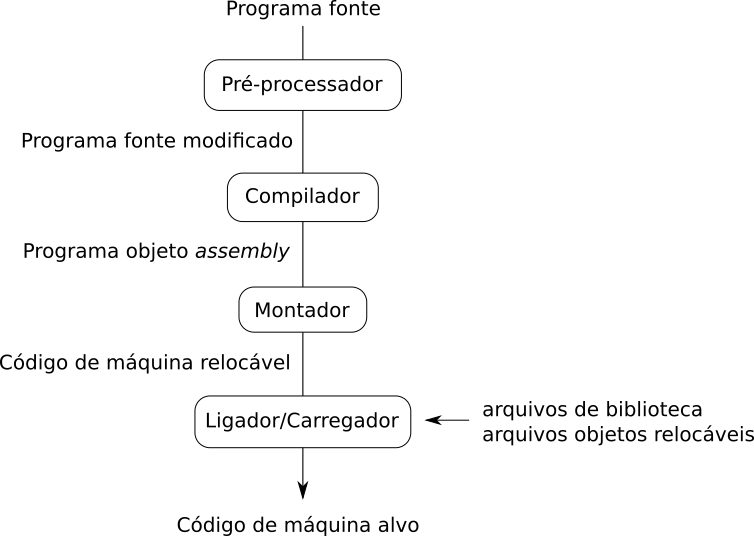
\includegraphics[width=\linewidth,height=\textheight,keepaspectratio]{figuras/programasrelacionados.png}
\end{frame}

\begin{frame}
   \frametitle{Exemplo de Compilação - Programa em C}
   \begin{itemize}
      \item Vamos compilar um simples programa em C para entender as etapas;
      \item considere uma pasta \textit{projeto} com o seguinte conteúdo:
      \begin{itemize}
         \item Subdiretório \textit{include} com o arquivo \textit{biblioteca.h};
	 \item subdiretórios \textit{lib} e \textit{bin} vazios;
	 \item subdiretório \textit{src} com os arquivos \textit{main.c} e \textit{biblioteca.c}.
      \end{itemize}
      \item nós vamos criar uma biblioteca e usá-la em um programa principal;
      \item a divisão do programa em vários arquivos é regra em programas não triviais.
   \end{itemize}
\end{frame}

\begin{frame}[fragile]
   \frametitle{Exemplo de Compilação - Programa em C}
   \begin{minted}{c}
/*** Conteúdo de biblioteca.h ***/
void funcao_da_biblioteca();

/*** Conteúdo de biblioteca.c ***/
#include <stdio.h>
void funcao_da_biblioteca() {
   printf("Olá Mundo da Biblioteca.\n");
   return;
}

/*** Conteúdo de main.c ***/
#include <stdio.h>
#include "biblioteca.h"
int main(int argc, char *argv[]) {
   funcao_da_biblioteca();
   return 0;
}
   \end{minted}
\end{frame}

\begin{frame}
   \frametitle{Exemplo de Compilação - Programa em C}
   \begin{itemize}
      \item O exemplo é trivial, mas já envolve muitos passos;
      \item um programa complexo, com centenas de arquivos fonte, compilado da forma que vamos mostrar seria impraticável;
      \item a maioria utiliza ferramentas (\textit{autoconf}) para automatizar a compilação:
      \begin{enumerate}
         \item Informações sobre o ambiente são inseridas em um arquivo de configuração;
	 \item um \textit{script} chamado \textit{configure} realiza testes e coleta mais informações sobre o sistema;
	 \item o comando \textit{make} invoca o compilador várias vezes para construir o projeto.
      \end{enumerate}
      \item porém, não é o foco da disciplina apresentar as ferramentas \textit{autoconf}.
   \end{itemize}
\end{frame}

\begin{frame}[fragile]
   \frametitle{Exemplo de Compilação - Programa em C}
   \begin{minted}{bash}
$ cd projeto
$ gcc -Iinclude/ -c src/main.c -o bin/main.o
$ gcc -Iinclude/ -c src/biblioteca.c -fPIC\\
-o bin/biblioteca.o
$ gcc -shared bin/biblioteca.o -o lib/libbiblioteca.so
$ gcc bin/main.o -Llib/ -lbiblioteca -o bin/a.out
$ bin/a.out
bin/a.out: error while loading shared libraries
$ LD_LIBRARY_PATH=lib/ bin/a.out 
Olá Mundo da Biblioteca.
   \end{minted}
\end{frame}

\section{Fases da Compilação}

\begin{frame}
   \frametitle{As Fases de um Compilador}
   \centering
   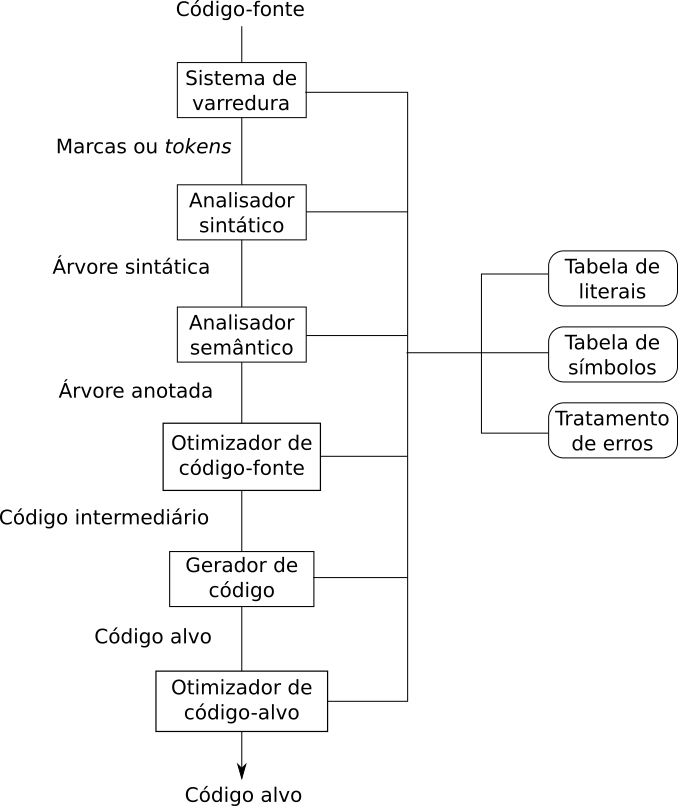
\includegraphics[scale=0.35]{figuras/etapas.png}<1>
   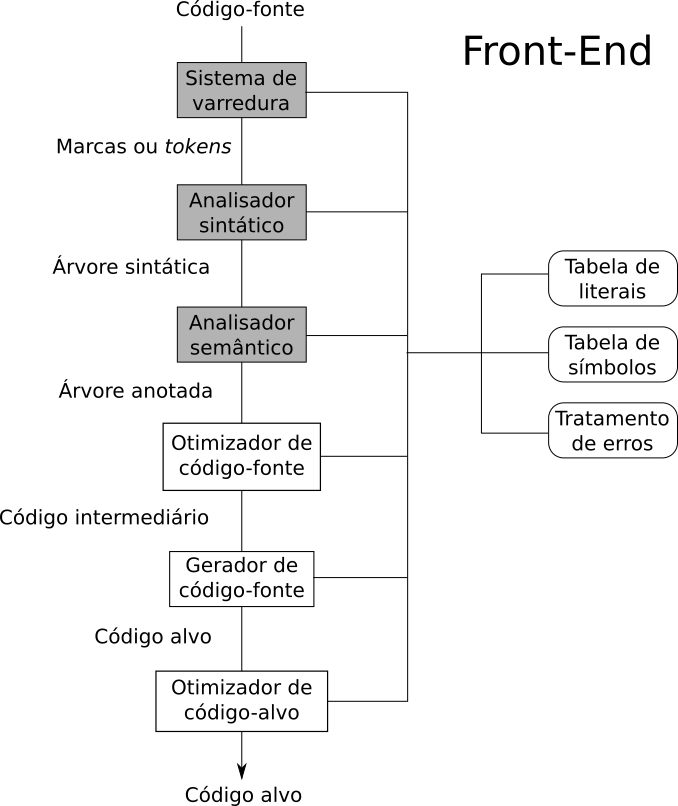
\includegraphics[scale=0.35]{figuras/etapasfrontend.png}<2>
   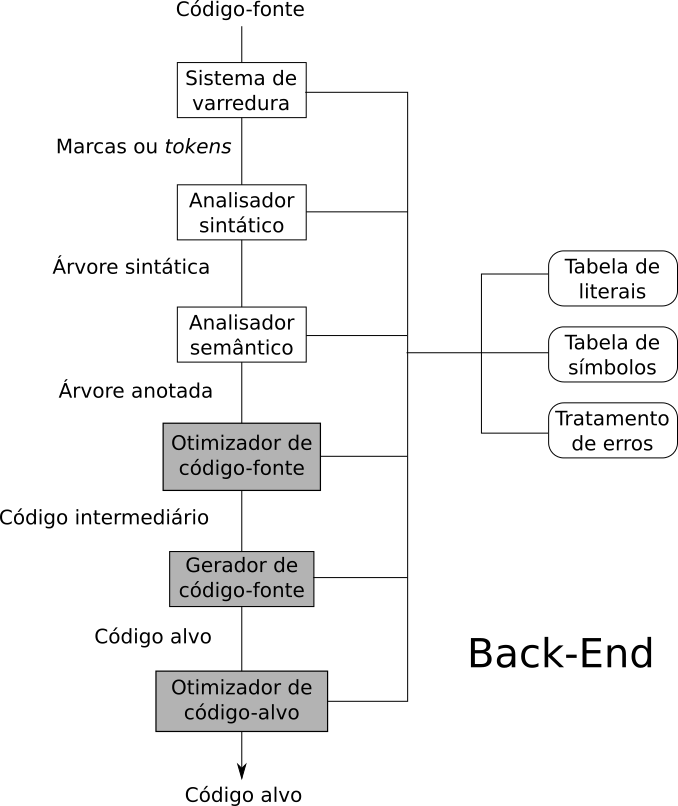
\includegraphics[scale=0.35]{figuras/etapasbackend.png}<3>
\end{frame}

\begin{frame}[fragile]
   \frametitle{Varredura ou Análise Léxica}
   \begin{block}{Marcas ou \textit{tokens}}
   Sequências de caracteres organizadas como unidades significativas.
   \end{block}
   \begin{minted}{c}
   a [index] = 4 + 2     
   \end{minted}
   \begin{table}
      \begin{tabular}{c|c}
      Símbolo & \textit{Token} \\
      \hline 
      a     & identificador \\
      $[$   & colchete à esquerda \\
      index & identificador \\
      $]$   & colchete à direita \\
      =     & atribuição \\
      4     & número \\
      +     & sinal de adição \\
      2     &  número \\
      \end{tabular}
   \end{table}
\end{frame}

\begin{frame}
   \frametitle{Analisador Sintático}
   \begin{block}{Árvore sintática}
   Determina os elementos estruturais do programa e seus relacionamentos.
   \end{block}
   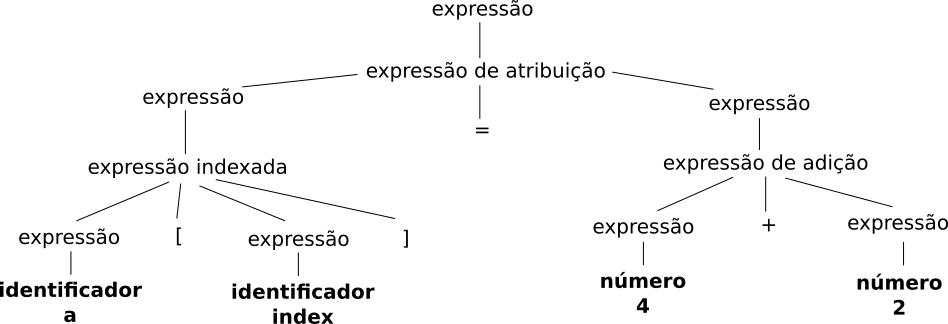
\includegraphics[width=\linewidth,height=\textheight,keepaspectratio]{figuras/arvoresintatica.png}<1>
   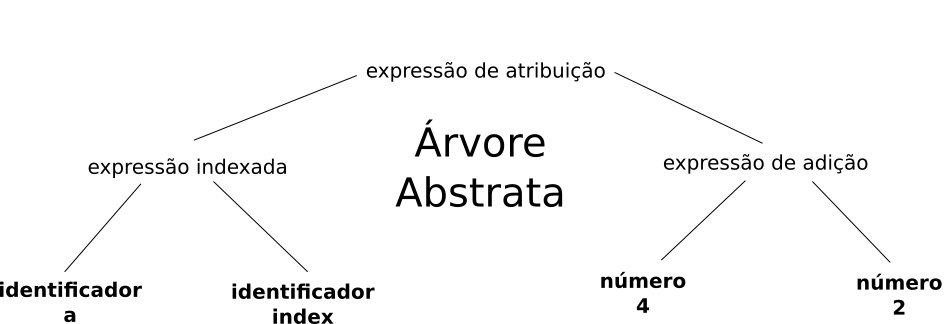
\includegraphics[width=\linewidth,height=\textheight,keepaspectratio]{figuras/arvoresintaticaabstrata.png}<2>
\end{frame}

\begin{frame}
   \frametitle{Analisador Semântico}
   \begin{block}{Verificação de Tipos}
   Consistência do programa em relação aos tipos empregados.
   \end{block}
   \vspace{1.0cm}
   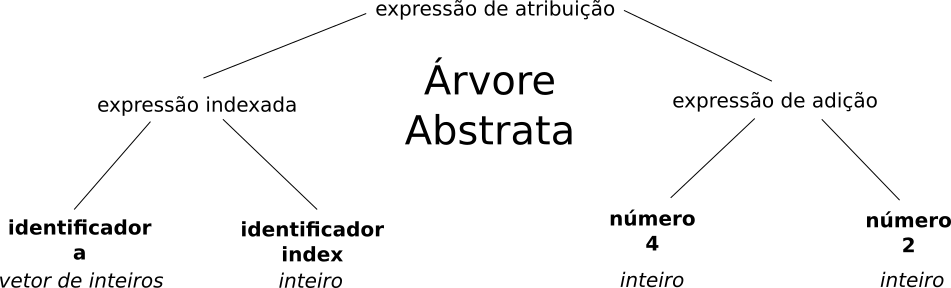
\includegraphics[width=\linewidth,height=\textheight,keepaspectratio]{figuras/arvoresemantica.png}
\end{frame}

\begin{frame}[fragile]
   \frametitle{Otimizador de Código-Fonte}
   \begin{block}{Otimizações à Nível da Linguagem de Alto Nível}
   Aplicar técnicas padrão de melhoria no código.
   \end{block}
   \begin{columns}
      \begin{column}{0.3\textwidth}
         \footnotesize
         \begin{minted}{c}
   // Original
   t = 4 + 2;
   a[index] = t;

   // Primeiro passo
   t = 6;
   a[index] = t;

   // Segundo Passo
   a[index] = 6;
         \end{minted}
      \end{column}	 
      \begin{column}{0.8\textwidth}
         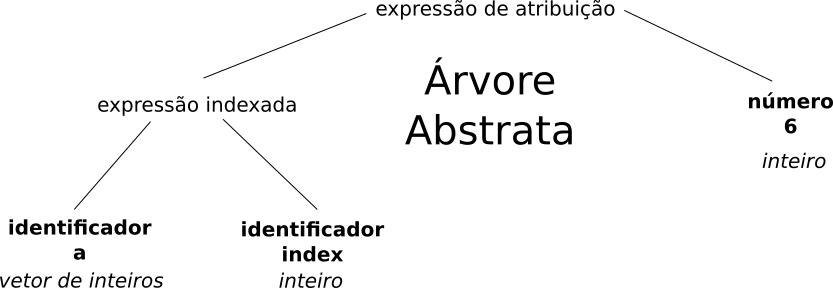
\includegraphics[scale=0.3]{figuras/otimizadorcodigofonte.png}
      \end{column}	  
   \end{columns}
\end{frame}

\begin{frame}[fragile]
   \frametitle{Gerador de Código}
   \begin{block}{Código Objeto}
   A partir do código intermediário, gera o código objeto. (Obs: Mostramos código de montagem por fins didáticos).
   \end{block}
   \begin{minted}{c}
MOV R0, index  ;; valor de index para R0   
MUL R0, 2      ;; dobra o valor em R0
MOV R1, &a     ;; endereço de a para R1
ADD R1, R0     ;; adiciona R0 a R1
MOV *R1, 6     ;; constate 6 para o endereço em R1
   \end{minted}
\end{frame}

\begin{frame}[fragile]
   \frametitle{Otimizador de Código-Alvo}
   \begin{block}{Melhorias no Código Objeto}
   Tira proveiro de características da arquitetura.
   \end{block}
   \begin{minted}{c}
MOV R0, index ;; valor de index para R0
SHL R0        ;; dobra o valor em R0
MOV &a[R0], 6 ;; constante 6 para endereço a + 10
   \end{minted}
\end{frame}

\section{Estruturas de Dados de Suporte}

\begin{frame}
   \frametitle{Estruturas de Dados}
   \begin{block}{Marcas ou \textit{Tokens}}
   Descrição do símbolo e cadeia de caracteres associada.
   \end{block}

   \begin{block}{Arvóre Sintática}
   Cada nó é um registro com atributos sintáticos e semânticos.
   \end{block}

   \begin{block}{Tabela de Símbolos}
   Identificadores de funções, variáveis, constantes e tipos de dados.
   \end{block}
\end{frame}

\begin{frame}
   \frametitle{Estruturas de Dados}
   \begin{block}{Tabela de Literais}
   Constantes e cadeias de caractares.
   \end{block}

   \begin{block}{Código Intermediário}
   Estrutura de vida curta que permite manipulações para otimizações.
   \end{block}

   \begin{block}{Arquivos Temporários}
   Quando a memória era pequena, arquivos eram utilizados para armazenas as estruturas do compilador.
   \end{block}
\end{frame}

\section{Questões de Projeto}
\begin{frame}
   \frametitle{Questões de Projeto}
   \begin{itemize}
      \item Análise e síntese;
      \item frente e fundo;
      \item passadas;
      \item definições de linguagens;
      \item opções e interfaces de um compilador;
      \item tratamento de erros.
   \end{itemize}
\end{frame}

\section{Compilação Cruzada}
\begin{frame}
   \frametitle{Reflexões}
   \begin{itemize}
      \item Em qual linguagem foi feito o primeiro compilador C?
      \item Em qual linguagem são escritos os compiladores C da atualidade?
      \item O compilador Java, é escrito em qual linguagem?
      \item A máquina virtual Java, é escrita em qual linguagem?
      \item Se vou instalar um sistema em um sensor ou sistema embarcado, devo compilar o código no sensor/sistema?
   \end{itemize}
\end{frame}

\section{A Linguagem TINY}

\begin{frame}
   \frametitle{A Linguagem TINY}
   \begin{itemize}
      \item Um curso de compiladores poderia mostrar como construir um compilador de C para a arquitetura x86-64;
      \item seria cansativo para o professor;
      \item os alunos teriam que ter alto conhecimento da especificação de C e de instruções x86-64;
      \item o índice de reprovação seria alto!
   \end{itemize}
   \begin{block}{Solução}
   Utilizar uma linguagem de programação \textit{brinquedo} para exercitar os conceitos: TINY.
   \end{block}
\end{frame}

\begin{frame}[fragile]
   \frametitle{A Linguagem TINY}
   \begin{minted}{c}
   { Exemplo de programa em TINY - fatorial }
   read x; { inteiro de entrada }
   if x > 0 then { não calcula se x <= 0 }
      fact := 1;
      repeat
         fact := fact * x;
	 x := x - 1;
      until x = 0;
      write fact { apresenta o fatorial de x }
   end
   \end{minted}
\end{frame}

\begin{frame}
   \frametitle{A Máquina TM}
   \begin{itemize}
      \item Mesmo para uma linguagem simples como TINY, gerar código x86-64 é árduo;
      \item a solução novamente é adotar uma máquina \textit{brinquedo} hipotética;
      \item a máquina TM possui apenas instruções básicas, sendo de compreensão mais acessível;
      \item novamente, trabalhamos com linguagem de montagem para facilitar a compreensão, mas a maioria dos compiladores produz código objeto.
   \end{itemize}
\end{frame}

\begin{frame}[fragile]
   \frametitle{A Máquina TM}
   O código  a[index]=6; equivale a:
   \footnotesize
   \begin{minted}{c}
LDC   1,0(0)    coloca 0 no registrador 1
* a instrução abaixo assume que o índice (index)
* está no endereço 10 da memória
LD    0,10(1)   coloca valor de 10 + R1 no registrador R0
LDC   1,2(0)    coloca 2 no registrador R1
MUL   0,1,0     coloca R1 * R0 em R0
LDC   1,0(0)    coloca 0 no registrador R1 
* a instrução abaixo assume que a variável a está no
* endereço 20 da memória
LDA   1,20(1)   coloca 20 + R1 no registrador R1
ADD   0,1,0     coloca R1 + R0 no registrador R0
LDC   1,6(0)    coloca 6 no registrador R1
ST    1,0(0)    armazena o valor de R1 no endereço 0+R0
   \end{minted}
\end{frame}

\section*{Dúvidas}
\begin{frame}
   \frametitle{Dúvidas?}
   Dúvidas ou comentários?
\end{frame}

\end{document}
